
%proof version
%\documentclass{gji}
%draft version

\documentclass{gji}

%\usepackage[backend=biber,natbib]{biblatex}
\usepackage{timet}

\usepackage{gensymb}
\usepackage{xargs}                      % Use more than one optional parameter in a new commands
\usepackage[pdftex,dvipsnames]{xcolor}  % Coloured text etc.
\usepackage{ulem}						% Allows sout option

\usepackage[colorinlistoftodos,prependcaption]{todonotes}
\newcommandx{\done}[2][1=]{\todo[author= Done ,linecolor=OliveGreen,backgroundcolor=OliveGreen!25,bordercolor=OliveGreen,#1]{#2}}
\newcommandx{\unsure}[2][1=]{\todo[caption={unsure},linecolor=gray,backgroundcolor=gray!25,bordercolor=gray,#1]{#2}}

%\usepackage{natbib}

\usepackage[colorlinks=true, allcolors=blue]{hyperref}

\title[Localization of the maximum acoustic coupling zone]
  {}
\author[F. Zedek L. Rolland et al.]
  {F. Zedek$^1$\thanks{Pacific Region Office, GJI}, L. Rolland$^1$ et al. \\
Affiliation Geoazur
  }
\date{Received ; in original form }
\pagerange{\pageref{firstpage}--\pageref{lastpage}}
\volume{xxx}
\pubyear{20xx}

%\def\LaTeX{L\kern-.36em\raise.3ex\hbox{{\small A}}\kern-.15em
%    T\kern-.1667em\lower.7ex\hbox{E}\kern-.125emX}
%\def\LATeX{L\kern-.36em\raise.3ex\hbox{{\Large A}}\kern-.15em
%    T\kern-.1667em\lower.7ex\hbox{E}\kern-.125emX}
% Authors with AMS fonts and mssymb.tex can comment out the following
% line to get the correct symbol for Geophysical Journal International.
\let\leqslant=\leq

\newtheorem{theorem}{Theorem}[section]
%--------------------------------
\begin{document}
%---------------------------------

\label{firstpage}

\maketitle


\begin{summary}
  subduction zones -> below water = hard to study
     would be helpfull to have more data
            -> idea : use TID produced by the event in near(semi) field 
    We study the potential of this method to constraint the uplift zone with 30s data 
    Study : Pedernales 2018/04/16 

LEs données 1S apportent quoi en plus ? (idee voir les pointés de temps arivées)

Subduction zones are at the origin of the largest earthquakes and instrumentted them remains difficult because most of them are located under the oceans. Thus, classical onland instrumentation (GPS, seismology, InSAR...) does not allow certain parameters to be well resolved, such as the spatial extent of the rupture or the size of the tsunami that generally follows. One solution could come from studying the disturbances generated in the surrounding ionosphere by the event, earthquake and/or tsunami. These ionospheric disturbances result from coupling between land envelopes and can be tracked even over the oceans using ground-based GPS stations. We studied the potential of these ionospheric signals to constrain vertical uplift zones at the source. We focused in particular on a recent and well-documented earthquake, known as the Pedernales earthquake (Mw 7.8, Ecuador) of April 16, 2016, and whose rupture is mostly undersea.

enjeux imager source tsunamis


\unsure[inline]{Based on a parametric study, we show that ionospheric disturbances are mainly sensitive to the maximum uplift zone. But, the parameters of the model to take into account for a fine reconstruction of the observation are, in addition to its location, its initiation time, its amplitude and also the duration of the acoustic pulse associated with the uplift. This sensitivity of ionospheric data suggests an innovative use, especially since the approach is based on an existing, widespread, inexpensive and rapidly expanding technology. }
\todo[inline]{add the 30s part}
\todo[inline]{Florian's drive \url{https://drive.google.com/drive/folders/1V_BZK6es4G_p5GqnUbO_sK62iUpSy0hi?usp=sharing}}
\end{summary}

\begin{keywords}
 GNSS, Ionosphere, Sismology, Modelisation, Acoustic Source
\end{keywords}
 \done[inline]{copy abstract from M2 report in SUMMARY part}
\done[inline,caption={installer le correcteur orthographique LanguageTool pour verifier l'anglais}]{installer le correcteur orthographique LanguageTool pour verifier l'anglais, voir ici \url{https://www.overleaf.com/help/334-can-i-use-overleaf-with-language-checking-tools-such-as-grammarly\#.W2wNwrg6-Uk}}
 
 
\todo[inline]{N shape : see Chum, 2016 }
 
 
%      ______________________________________________________________________________
% 	 /		       				     	Introduction                                  \
%	/__________________________________________________________________________________\
%	\  establishing a territory (In the past decade much research has focused on...)   /
%	  \            -------------------------------------------------------	         /	
%	    \		 	   establishing a niche (it remains unclear...)                 /
%	      \          ---------------------------------------------------	       /
%		   \			Occupying the niche (the purpose of this study is...)    /
%	         \ __   ---------------------------------------------------	    __ /
%			     \				 Literature review                        /
%			       ------------------------------------------------------
 
 
 
\section{Introduction}

\fbox{\begin{minipage}{1\linewidth}
problematic :   Describe importance to monitor eq and subduction zone
 
   State of the art
          see  heki 2018 
        [olson, 1957] : eq. provokes acoustic vibration as loudspeaker 
        [ ] couplage terre/eau/atmo 
        [ ] : N-shape 
        [Calais, 1995] : use GNSS to study it 
        [heki , 2005] : 
[????] : relation between uplift and acoustic source
        [ Astafyeva 2011 ]  the wave shape is linked to the magnitude
        [ Rolland 2011 ] we are able to reconstruct the directivity of the perturbation knowing the GNSS satellite position and the magnitic field above the rupture
        [Lee, 2018] the localisation of the acoustic source is important when we try to reconstruct the arrival time of the perturbation. moreover we cannot place the acoustic source at the epicentre for all eq. 

 what can we do :  help select a rupture model / ground displacement
*what is the sensitivity of Seismic CID to model  parameters ?

  \todo[inline]{Why is it important ?}
 \todo[inline]{State of the art}
See \cite{Heki2018} for a review of the properties of ionospheric disturbances triggered by earthquakes.
\done[inline]{Lire Heki (2018)}
\todo[caption={Lee et al. (2018) as a starting point},inline]{Report main lessons learned from Lee et al. (2018), and describe why and how they are used as a starting point.}
 \begin{itemize}
 \item few words on earth/atmosphere
 \item atmosphere ionosphere
 \item CID and detection
 \end{itemize}
 \end{minipage}}
 \newline
 ~
\newline
During the past two decades it became quite common to use Global Navigation Systems (GNSS) to monitor the ionospheric Total Electron Content (TEC) in order to retrieve the Coseismic-Ionospheric-Disturbance (CID) signal of an earthquake. The method first describe by Calais \& Minster \shortcite{Calais1995} consist in the use of a dual frequency GNSS receiver 

Shallow

Astafyeva, et al 2018 "CID generation over the epicentral area is not yet quite sufficient."


\begin{table}
    \begin{tabular}{c|cc|cccccc}
    			& \multicolumn{2}{c|}{ Modele} & \multicolumn{6}{c} {earthquake} \\
                
  parametre 	& A & b & uplift  & lon &lat & Mw & Heure (LT) & F10.7 \\ \hline 
   Van (2011-10-23)			&1.2	&  0.04 &	1.0 m	& 43.51 E & 38.72 N & 7.1 & 13:37 & 156	\\
   
   Kaïkoura (2016-11-13) 	&	1    &  0.06 &	8/4 m &		173.05 E	& 42.74 S	& 7.8 & 22:35 & 78	\\
   Sanriku (2011 - 03 - 09) 	& 1.5	&  0.04 &	0.3 m &	142.84 E	&		38.42 N	&	7.3& 11:45 & 143\\
   	
   Pedernales(2016-04-16)	& 5 	& 0.06  &	1.3 m&		79.92 W	&	0.38 N		& 7.8 & 18:38 &113 \\
   
\end{tabular}\\
  \caption{ review of parameter used for previous study }
    \label{recapparametres}
\end{table} 


\section{case Study}
	\subsection{pedernales earthquake} 
	\todo[inline]{       
        presentation of pedernales DD:HH, -\\ epicentre, focal mechanism, rupture size ...
        +reseaux GPS/available data
        }
the Pedernales earthquake that took place in the seismic zone around
of Ecuador-Colombia caused by the subduction of the Nazca oceanic plate under the
North Andean Silver (NAS) plate (Figure 6). We also see on this figure that Ecuador is
equipped with a GPS network whose initial purpose is to observe tectonic deformations and
volcanism in this region. In this area, considering as a fixed reference the plate
South American, the displacement of the Nazca plate is 8 to 11 mm per year towards the
Northeast (Nocquet et al., 2014) causing strong earthquakes.
On April 16, 2016 in Ecuador at 23:58 GMT (18:28 LT) there was an earthquake of magnitude
7.8 near the coastal town of Muisne (the epicentre being located at 0.38 $\deg$ North and -79.92 $\deg$ East according to
USGS), causing considerable damage, near the town of Pedernales, 55 km away
further south. The reverse fault failure (azimuth 29 $/deg$, dip 23 $\deg$) occurs over 100 km long for 40 km wide at a depth of 15 to 30 km over a period of 48 seconds. The
rupture spread southward with a cumulative peak slip on the fault estimated at 7
meters, which produced a maximum vertical displacement of 1.2 m reaches about 30 seconds
after the initiation of the rupture (see Figure ). The data used for this estimate are
from accelerometers and High Rate GPS (HRGPS) presented in fig.are p.

        
        
\begin{figure}
\begin{center}
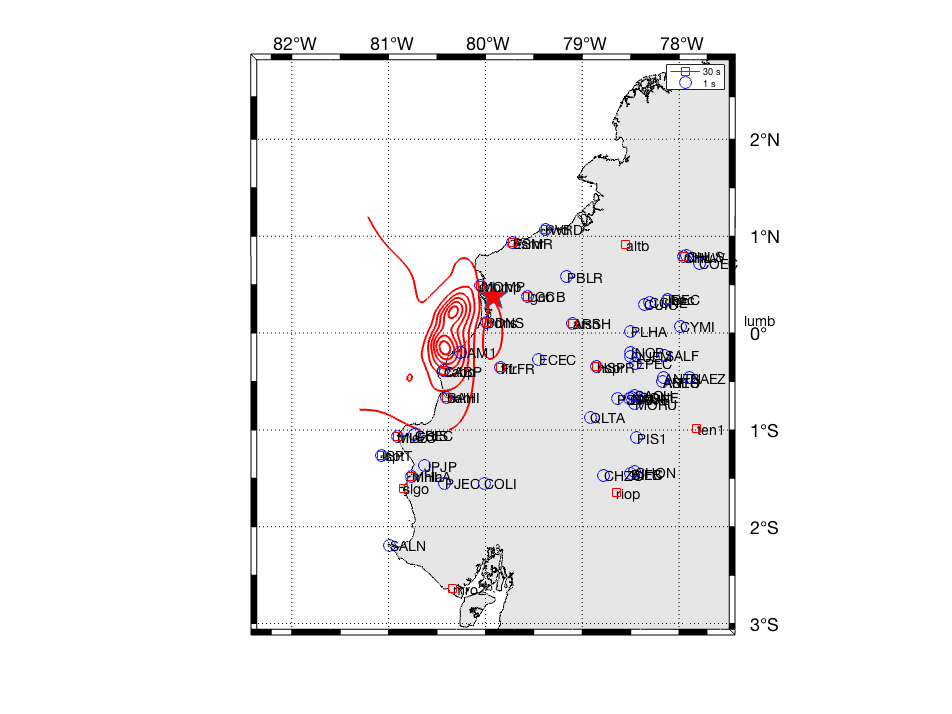
\includegraphics[width=1\linewidth]{images/ped1S30S.png}
attention : in legend 30s 1s are inverted\\
add fault plan \\
add ipp 
\end{center}
\caption{  Pedernales eq. the pedernales region , the rectangle is the fault plan (calculated by the USGS) The red square are the available 1s rate stations when the blue circles are 30s one. The magenta, cyan and blue respectively show the satellites tracks projected on ground for G06, G07 and G30 if the epicenter was a station from 10 min before the rupture to 30 min after ?(maybe just 10 or 20') }
\label{SituationMap}
\end{figure}
probably mixed with :

\begin{figure}
\begin{center}
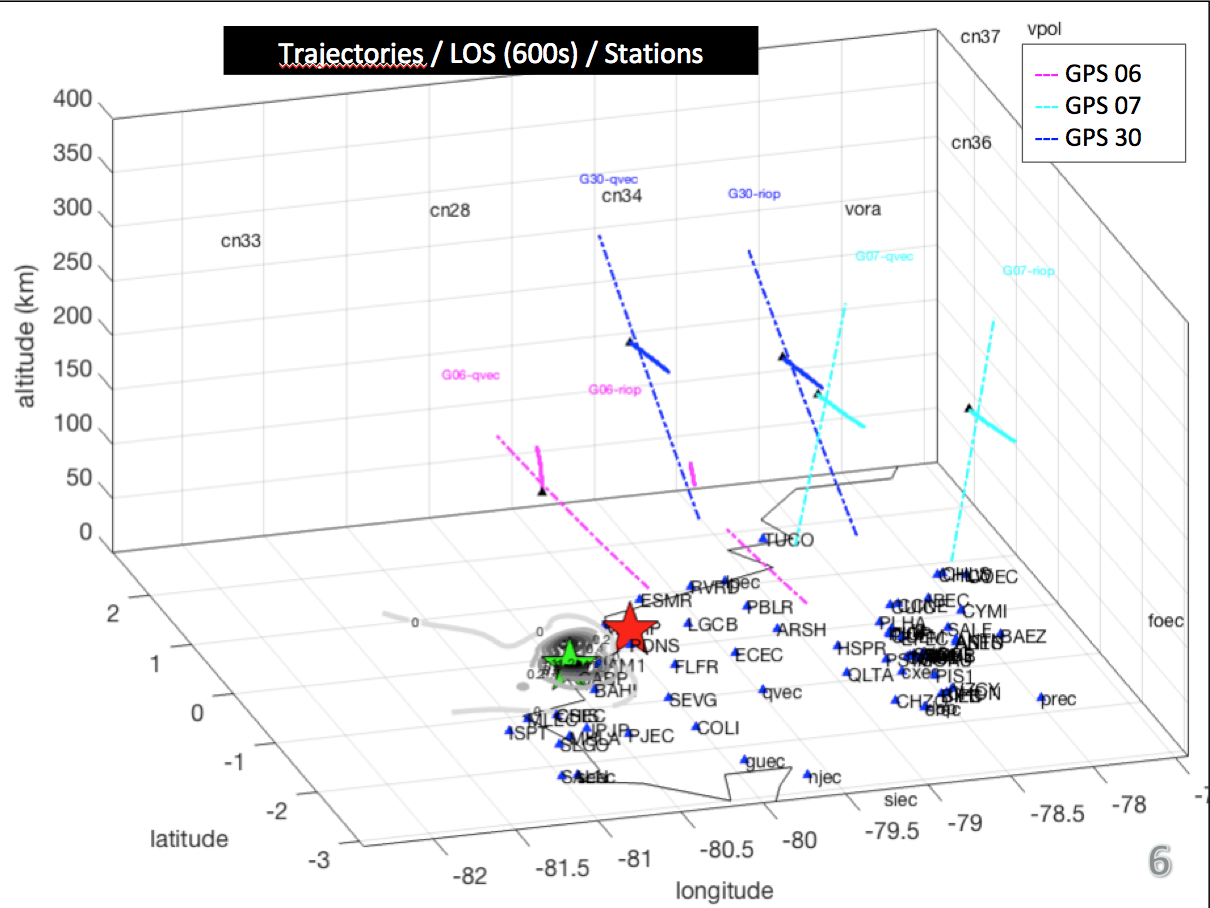
\includegraphics[width=1\linewidth]{images/situation_map_3D.png}
\end{center}
\caption{ \textit{\emph{3D view of the observation configuration for RIOP and QVEC stations}. The blue triangles identify the positions of the GPS stations. The IPP trajectories of these two stations observing satellites G06, G07, G30 are plotted assuming an ionospheric thin film at 300 km altitude and are represented in magenta, cyan and blue respectively. The black triangles indicate the position of the satellites 10 minutes before the earthquake, each black line represents the LOS between the satellite and the station between 150 and 400 km above sea level. The epicentre is symbolized by a red star, the maximum vertical displacement by a green star (1.2 m) and the contours represent the vertical displacement of the ground according to Nocquet's model (2016)}} 

%\end{center}
\label{superplot3D}
\end{figure}


	\subsection{observation geometry / IPP}
	In order to retrieve the ionospheric perturbation we used the ecuatorian gps network at 1s and 30s \todo[inline]{ask Jean-mathieu or Paul how to cite it} we select the satellites whom line of sight (LOS) cross the bottom of the ionosphere at a maximum of the 350 km (500) from the studied station in a time window from 10 minutes before the rupture to 20 minutes after it. We called this point the Sub-Ionospheric Pierce Point (SIPP) and choose its height at 180 km.
	\subsection{observation's extraction} 
       
       \paragraph{extract rinex Geometry free}
       
  \begin{equation}
Insert ~ geometry ~ free ~ equation
 \end{equation}
        \paragraph{filtrage / processing} 
        
        
            -region Map with satellite tracks\\
            - az/ele figure ?\\
            - Hodocrones (distance to SIPP)\\

\begin{figure}
 \begin{tabular}{l c r}
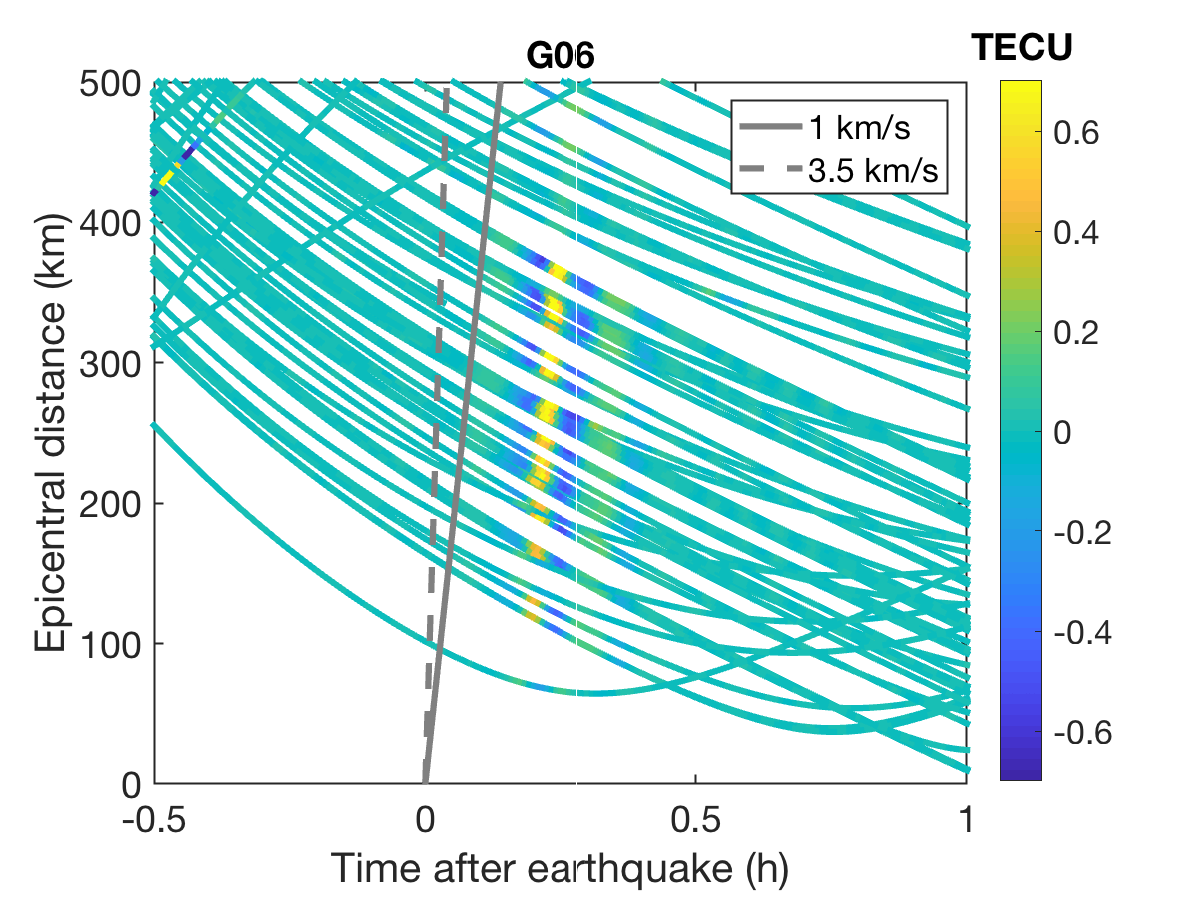
\includegraphics[width=0.3\linewidth]{images/hodocrone_G06.eps} & 
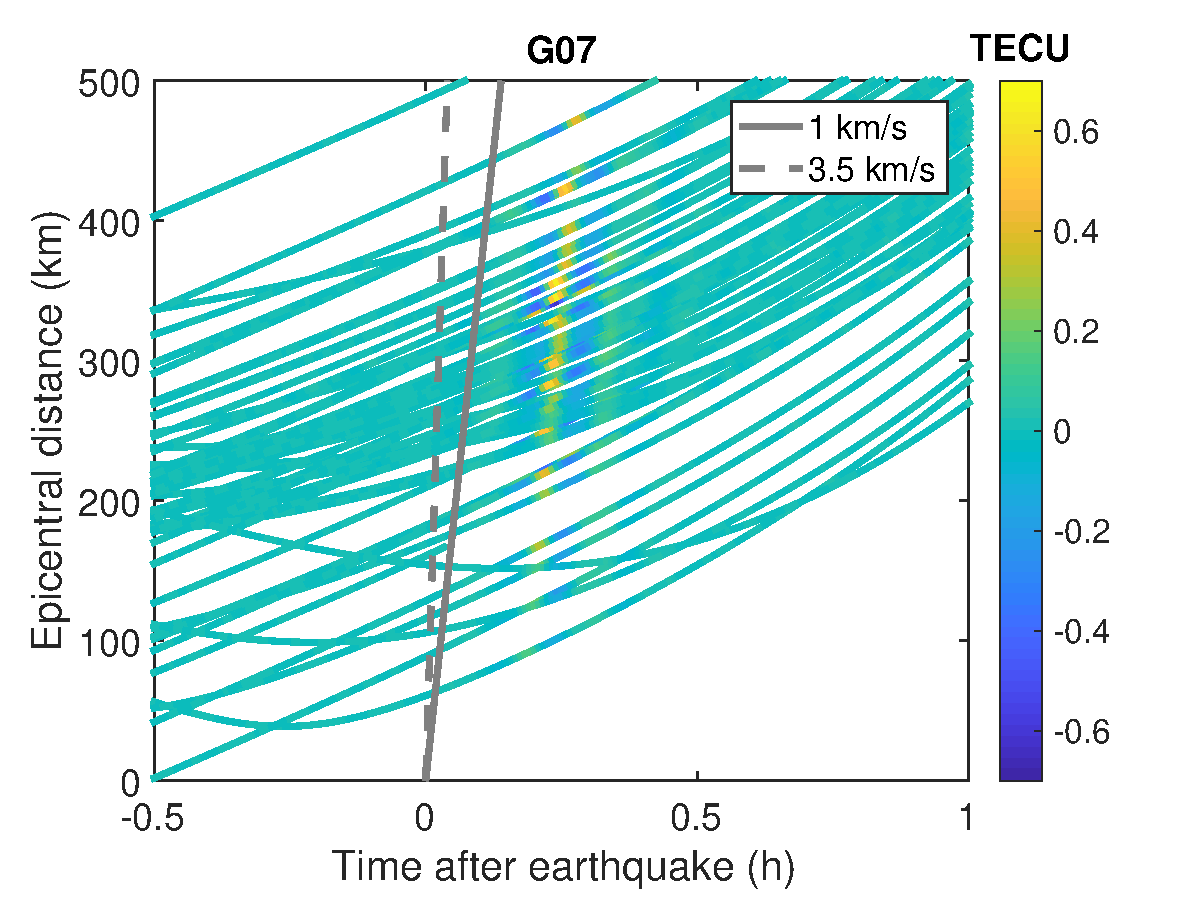
\includegraphics[width=0.3\linewidth]{images/hodocrone_G07.eps} &
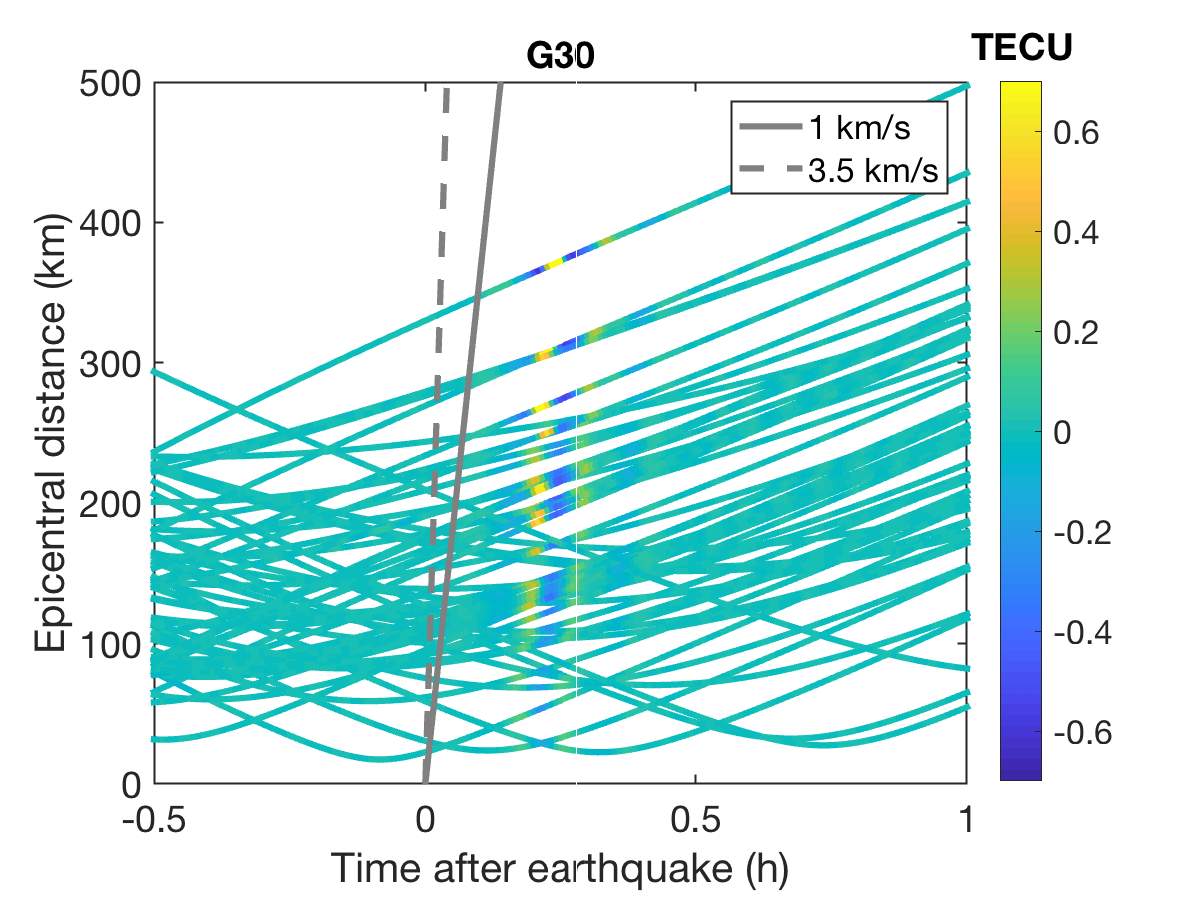
\includegraphics[width=0.3\linewidth]{images/hodocrone_G30.eps}
 
\end{tabular}
\caption{ Time/distance representation of TEC disturbance observations as a function of the distance between the SIP and the epicentre ("hodochrones"). The color scale indicates the amplitude of the filtered TEC  in TECu. The dashed grey line represents the expected arrival times for an acoustic wave propagating radially from the acoustic source at a speed of 3.5 km/s, speed of Rayleigh waves. The solid grey line corresponds to a speed of 1 km/s. }
\label{Hodochrone}
\end{figure}


\paragraph{atmospheric parameter}
\begin{figure}
\begin{center}
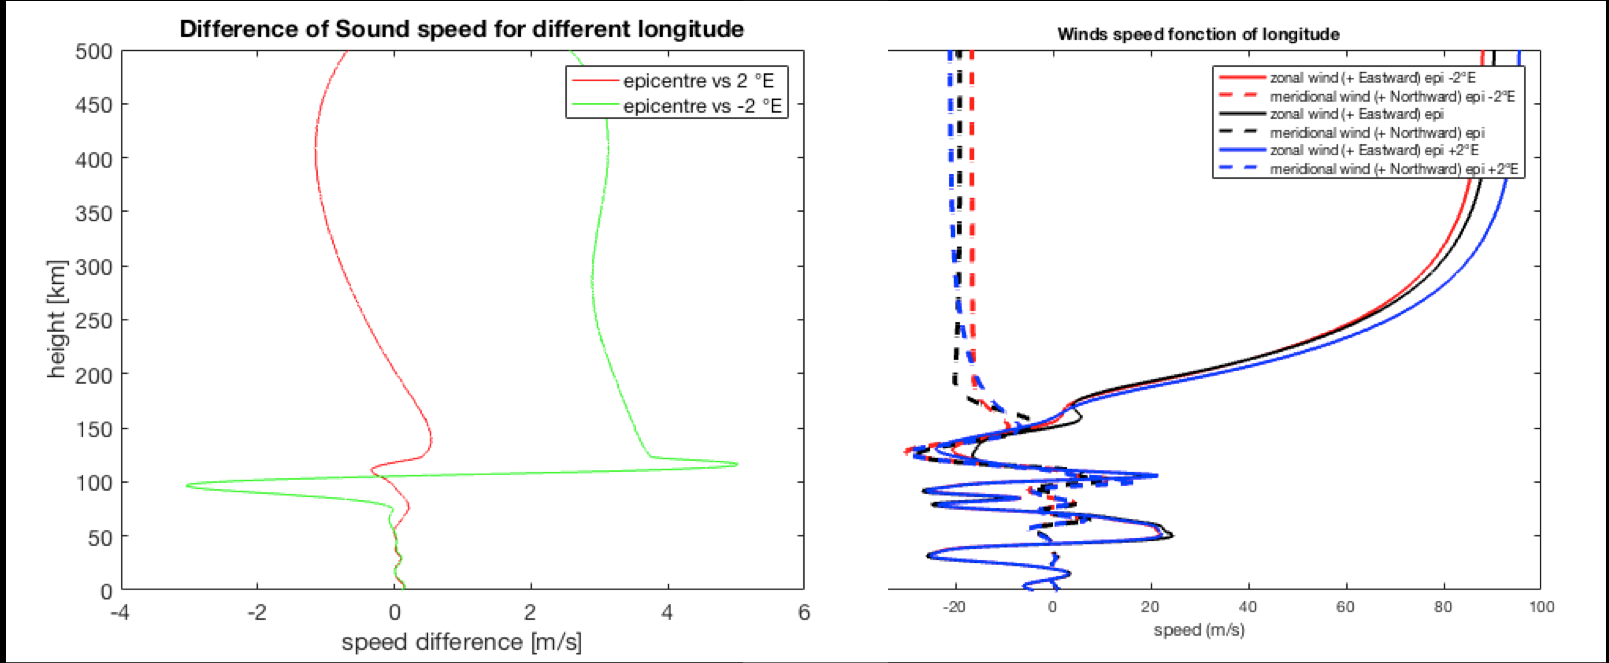
\includegraphics[width=1\linewidth]{images/sound_wind_epiVS2deg.png}
\end{center}
\caption{ \textit{\emph{atmospheric parameter}. a) sound speed for 2 different locations, b) wind speed for two different location }} 

%\end{center}
\label{atmos_param}
\end{figure}


%--------------------------------
% Methodology
%--------------------------------
\section{Modelisation} 
        Idea is to reconstruct the signal assuming N-shape wave produce in 1source point compute the perturbation for multiple receptor and found the acoustic source localisation where the perturbation is reconstructed the best. Following the methods proposed in Rolland et al. (2011,2013) we create an acoustic plane-wave centered on 5 mHz which follows the observed CID see ??? (citation). This wave is an N-shapes waves genreated from a gaussien derivative : 
      The impulse is an acoustic wave of 5 mHz propagating at sound speed, taking account of the attenuation 
      :\begin{equation}\label{fct_source}
V_p(t) = \frac{A\sqrt{2}}{\sigma^{\frac{3}{2}}\pi^{\frac{1}{4}}} (t-t_0) \ e^{-\frac{(t-t_0)^{2}}{2(\sigma)^{2}}} 
\end{equation}
        (-> eq N shape)
        (-> eq vitesse déplacement onde)
        
         This  acoustic wave is propagated in the atmosphere with a 3 Dimensional ray tracing method (citation, J.X. Dessa ?? + see details in quentin Brissaud thesis). Then the interaction between the waves and the atmospheric background is computed. The atmospherics parameters such as air density, temperature and sound speed are derived from NTRL (citation). We assume here a 1-D stratified atmosphere and the ionosphere background such as electron density is derived from IRI (citation) in 3-D. After that  the perturbation is integrated along the LOS between the SIPP at 180 ? (to discuss : astafyeva 2018, see changes if taking into account a lower boundary) and 500?? km of altitude in order to reconstruct the STEC perturbation. 
		\todo[inline]{check the acoustic cut-off frequency for this zone }   
		The synthetics are filtered with the same apodized butterworth filter than the observation.       
         
        As we plan to test the impact of the satellites position and especially its elevation on the data we kept the STEC instead of converting it to VTEC. Moreover as we reconstruct the perturbation in a specific geometry and compared it to the exact same geometry.
        \todo[inline]{add something in the discussion about the fact it seems not necessary to use VTEC in our case  }
        
        The main parameters we focused to tune in our work are in one hand the impact of the broadening factor in the N-Shape generated waves, in the other hand the localization of the acoustic source. We also apply an amplification factor to match the observed and the synthetic data which for now would be a non-sens to invert due to bad understanding of this parameter (see cahayadi 2016).
        \unsure[inline]{maybe a bit strong, check if cahayadi is the best quote or the other article where he try to inverte the amplitude.}

             -> we focused to study the tune of some parameter parameters which one can vary ?

    we models at epicentre and max uplift (hodoseries 1 or multi ?)
    
    \subsection{correlation}
to study the arrival time which assume that the time of maximum perturbation is well reconstruct and so the difference between the time of maximum perturbation in synthetics and observation gives us the delay of the model at one acoustic point source. The most accurate point source \sout{is} should be the one with the most station with small delay.
taking into account that seismological evidence shown that there is approx 30s between the rupture and the uplift ( well maybe thats a bit in advance , is there an article on it ?) 
\todo[inline]{get figure azimuth , distance for new grid point  : the file is in the drive and analyzed them a bit more}

    
   %---------------
   % results
   %---------------
   
\subsection{Forward Model}

finding b : a priori kaikoura  
the amplitude factor is not enough constraint to be calculated by himself and is adjust \begin{figure}

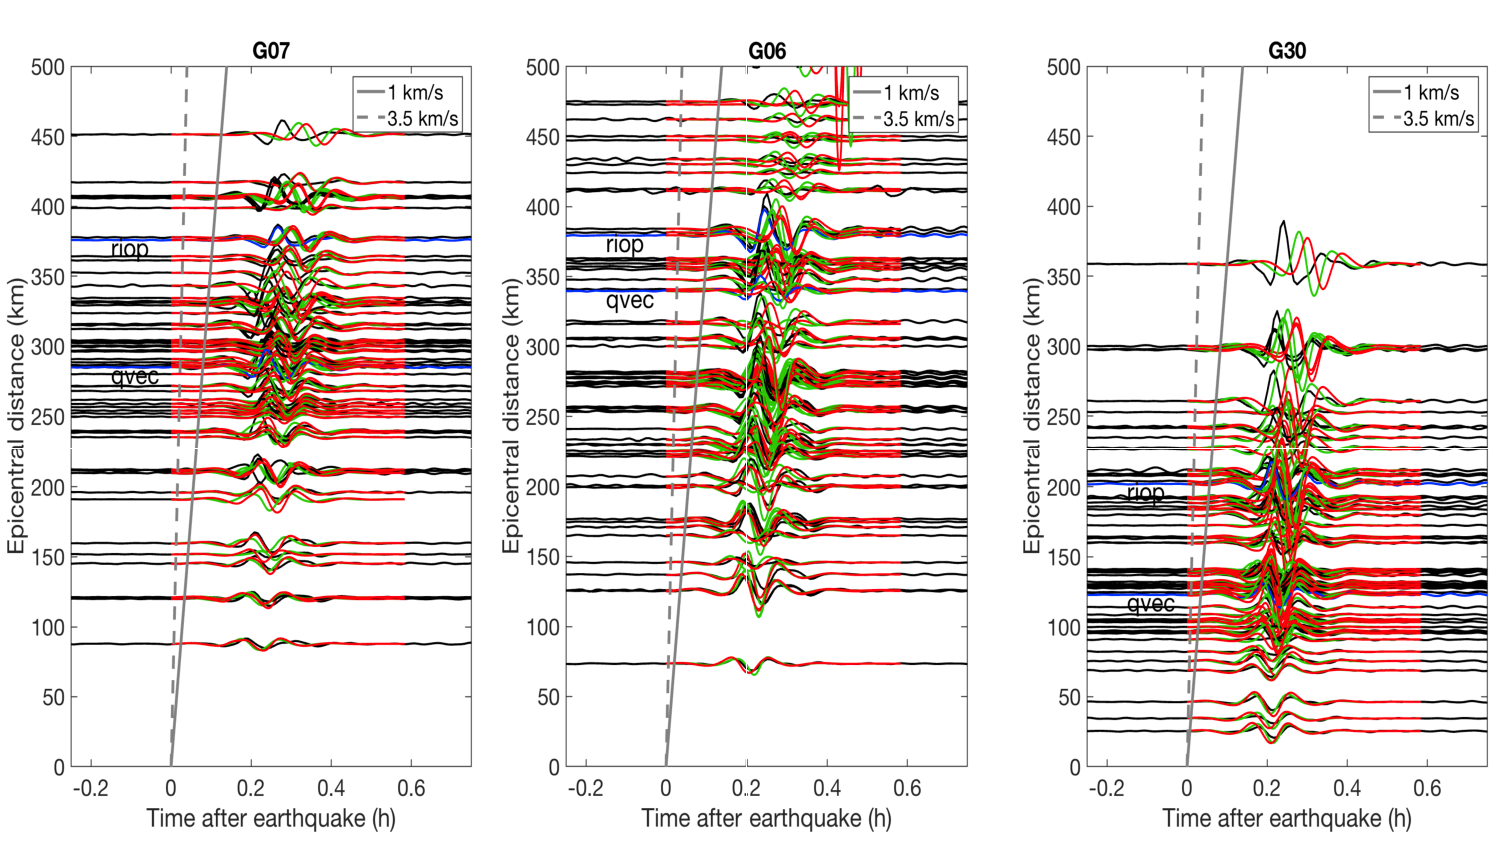
\includegraphics[width=0.9\linewidth]{images/Hodo_all_cropped.pdf}

redo with new version of IS \\
try with only 1s data\\
probably keep only one satellite
\caption{ \textit{\emph{observed and modelled TEC disturbance}.  Black curve: observed TEC disturbance, red curve: modelled disturbance with epicenter as source point, green curve: modelled disturbance with maximum vertical displacement as source point. In blue are marked the QVEC and RIOP stations. The grey line indicates the expected arrival times for an acoustic wave propagating radially from the acoustic source at a speed of 1 km/s.}}

\label{hodoseriesall}
\end{figure}
 \todo[inline]{rerun IS.V2 and estimate the correlation for different b, then chi2 to find A}

\section{Inversion}

*  scaling factor : finding A:  
                A(Value(maxcor))=Value(max(autocor))
*  finding b : b as low impact on amplitude so test for different b which one as the best correlation 
                    we used as start point kaikoura’s b to enhance speed


* definition of the correlation we use.
*  check the difference between syn and obs use FMNEAR
                (supplementary use of chi 2 to study phase?) 
    selection of parameter
        starting from the computed max uplift (Nocquet, 2016)
       
      
        when parameter are defined we launch the computation around the epicentre 4x4 degree grid with 0.5 degree step. we then select the area with the better correlation between mod and obs on a 0.1 degree grid, the selected area is … N …E ??
        
        
        \section{Results}
        
        
        
        * correlation MAP


\begin{figure}
 \begin{tabular}{l r}
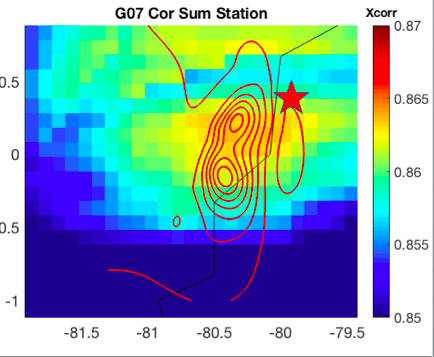
\includegraphics[width=0.44\linewidth]{images/cor_Map_G30_old.png} & 
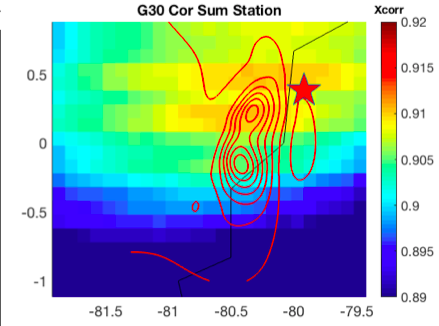
\includegraphics[width=0.50\linewidth]{images/cor_Map_G07_old.png}
 
\end{tabular}
\caption{ \textit{\emph{Correlation Map sum on sat G07 on the left and G30 on the right}.    }}
\label{Corr_Map}
\end{figure}





Results :
        We saw it exists a patch where the model better correlate the observation, this patch is similar to the one computed for NOCQUET et al. (2016) 

        1 time series with correlation, FMNEAR (2 station ?)
        
        
        \section{discussion}

        30 s data -> big eq. 
        A found really different A from previous study (give a world about the eq in case study / and here about previous ) 
        preferable satellite geometry 
        we used a narrow bandwidth filter we might loos info
table A
aliasing ?
filtrage ? 
identification de pb ? -> etudes stations 
conclusion : 
        this study show the huge potential of the modelisation of TEC perturbation after an eq
        
        %---------------------


\section{finding the best model}
From the epicenter location : we try to find the best parameters A and b \\
Then grid search around the epicentre from 2~\degree East to 2~\degree West and 2~\degree North to 2~\degree South with a 0.5~\degree step. Which means 81 acoustic source location. With selected b from 0.03 to 0.09 with a 0.01 step see \cite{Astafyeva2011} 
\todo[inline]{ cite Lee2018 Astafyeva2013}

\todo[inline,caption={bibtex Lee 2018}]{
% $@article{lee_kaikoura,	author = {Lee, Rebekah F and Rolland, Lucie M and Mikesell, T Dylan},doi = {10.1785/0120170299},isbn = {0120170299},issn = {0037-1106},journal = {Bulletin of the Seismological Society of America},month = {may},year = {2018},pages = {1--29},title = {Seismo{\-}Ionospheric Observations, Modeling, and Backprojection of the 2016 {Kaikōura} Earthquake},url = {https://pubs.geoscienceworld.org/ssa/bssa/article/530731/SeismoIonospheric-Observations-Modeling-and}\\ }
}
\todo[inline,caption={bibtex Astafyeva 2013}]{%$@article{astafyeva_parameters_2013,	title = {Parameters of seismic source as deduced from 1 {Hz} ionospheric {GPS} data: {Case} study of the 2011 {Tohoku}-oki event: {IMAGING} {OF} {SEISMIC} {SLIP} {FROM} {IONOSPHERE}},	volume = {118},	issn = {21699380},	shorttitle = {Parameters of seismic source as deduced from 1 {Hz} ionospheric {GPS} data},	url = {http://doi.wiley.com/10.1002/jgra.50556},	doi = {10.1002/jgra.50556},	language = {en},	number = {9},	urldate = {2018-06-13},	journal = {Journal of Geophysical Research: Space Physics},	author = {Astafyeva, E. and Rolland, L. and Lognonné, P. and Khelfi, K. and Yahagi, T.},	month = sep,	year = {2013},	pages = {5942--5950}}$
	}
    
    
In order to select the best parameters we study from three different way the differences and similarities between the model and the synthetics

\subsection{Amplitude factor}

Two methods were used to study the amplitude factor 

first we compare the maximum of STEC perturbation between synthetics and data
then we use for all station and use the root mean square method to obtain the best slopes for each satellite. The best is found for A $^+_-$ 4.5 
the best fit are found on 0.5 step grid with a correlation coefficient of : xx for a broadenning factor between 0.07 and 0.09 and localised xx

the other method is to compare the maximum of correlation between synthetics and observation as :
\begin{equation}
A ~ .~ max(correlation_{synthetics}) =  max(correlation_{observation})
\end{equation}

\todo[caption={discussion},inline]{discussion : As the broadening factor is ill-defined with the first method and as the broadening factor as a not so much impact on the amplitude for a given location we choose to not take it into account to select it (+ see Astafyeva2013)  }


\subsection{Chi2 derived}
\paragraph{Chi2 derived}
\begin{equation}
\chi^2 = \frac{1}{T}\sqrt{\sum_{t=1}^{T}\frac{(O_t-S_t)^2}{O_t^2 + S_t^2}} 
\end{equation}
With T the Total time en t the time of observation. O is the value observe and S the Synthetic value.

we found that the best was at a values of ... for GPS ... x3
other small values from 0... to 0.xx were on the area of lat / lon from the epicenter

We also try to use the mean amplitude factor we first found with A = 5 ,translated in the $\chi^2$ equation as the permutation of $O_t$ by $^5O _t = 5*O_t$. With this approach the smallest $\chi^2$ was found at ... x3 but other small chi in the range ... were found in the area ...

\todo[inline]{do the same with O/max(o) and S/max(S) => it's a quick work}

This method also allow us to compare $\chi2$ over the different broadening factor which sometimes modify the best acoustic source location from 1 step order between 2 following values of broadening factor. Smallests $\chi^2$ are found between b=0.06 and 0.07 but at different location
    
\paragraph{RMS}
  an other $\chi^2$ derived formula to find the best fitting parameters was to use the Root mean square methods \todo[inline]{see Bertrand's paper FMNEAR}  
    \begin{equation}
    RMS= \frac{1}{T}\sqrt{\frac{\sum_{t=1}^{T}(O_t-S_t)^2}{\sum_{t=1}^{T} O_t^2 }} 
    \end{equation}
    
   \subparagraph{CHi2 0.1 degree}
   When zooming between lat : (-1.5:0.1:0.5)
lon(-2:0.1:0.5) with a step 0.1 the area for each GPS is now well define but is still different between two satellite
\todo[inline]{see florian drive : inversion smallgrid : chi2} 
    
 \label{lastpage}   
    
    
%-------------------------------------------------
% 				  SUPPLEMENTARIES
%_________________________________________________
 \newpage
 \section{supplementaries}
 \subsection{filtering}
 We study the effect of the filtering effect on the synthetics and the observation
 as the wave attenuation is centered on a 5~mHz frequency we try to apply a butter-worth filter around this values. Comparing a 0.5 to 10 mHz to a 2 to 8 mHz filter we saw the model is not able to reconstruct accurately the long-period term of the signal as it was possible for the Van earthquake of magnitude 7.1. the 0.5 to 2 mHz band seems to be able to provides more constraint on strong magnitude earthquake. 
 \todo[inline]{add figures}
 
  \bibliographystyle{gji}
 \bibliography{Mendeley}
 \listoftodos
 
 



\end{document}